\documentclass[twoside,a4paper,11pt]{article}
\usepackage[T1]{fontenc}
\usepackage{times}
\usepackage{elcvia}
\usepackage{elcvia-submission}
\usepackage[english]{babel}
\usepackage{amsmath,amssymb}
\usepackage{graphicx}
\usepackage{booktabs}
\usepackage[numbers,sort&compress]{natbib}
\usepackage[hidelinks,breaklinks]{hyperref}
\usepackage{xurl}
\usepackage{placeins}
% Prevent isolated first or last paragraph lines at page breaks.
\clubpenalty=10000
\widowpenalty=10000
\renewcommand{\topfraction}{0.9}
\renewcommand{\bottomfraction}{0.8}
\renewcommand{\textfraction}{0.1}
\renewcommand{\floatpagefraction}{0.8}
\urlstyle{same}
% Break DOIs at their prefix separator, keeping identifier suffixes intact.
\newcommand{\doi}{doi: \begingroup\urlstyle{rm}%
  \def\UrlBreaks{\do\/}\def\UrlBigBreaks{\do\/}\Url}
\hypersetup{pdftitle={Supplementary Material: How Far Does Corruption Robustness Transfer? A Leave-One-Family-Out Study on CIFAR-100-C}}
\newif\ifblindreview
\ifdefined\ELCVIABlindReview\blindreviewtrue\else\blindreviewfalse\fi
\ifblindreview
\hypersetup{pdfauthor={}}
\else
\hypersetup{pdfauthor={Rakhman Seidigali and Yermakhan Khamitov}}
\fi

\title{Supplementary Material\\How Far Does Corruption Robustness Transfer?\\A Leave-One-Family-Out Study on CIFAR-100-C}
\author{Rakhman Seidigali and Yermakhan Khamitov\\[1ex]
\small\emph{School of Software Engineering, Astana IT University}\\
\small\emph{Astana, Kazakhstan}}
\date{}
% Generated from independently recounted v3 data. Do not hand-edit.
\newcommand{\GainNoiseMac}{15.87}
\newcommand{\GainNoiseMacSD}{1.14}
\newcommand{\GainNoiseMacLow}{14.45}
\newcommand{\GainNoiseMacHigh}{17.28}
\newcommand{\RefGainNoiseMac}{40.35}
\newcommand{\RefGainNoiseMacSD}{0.99}
\newcommand{\RefGainNoiseMacLow}{39.12}
\newcommand{\RefGainNoiseMacHigh}{41.58}
\newcommand{\GapNoiseMac}{-24.48}
\newcommand{\GapNoiseMacSD}{1.04}
\newcommand{\GapNoiseMacLow}{-25.77}
\newcommand{\GapNoiseMacHigh}{-23.19}
\newcommand{\RatioNoiseMac}{0.393}
\newcommand{\RatioPctNoiseMac}{39.3}
\newcommand{\GainBlurMac}{10.92}
\newcommand{\GainBlurMacSD}{0.69}
\newcommand{\GainBlurMacLow}{10.06}
\newcommand{\GainBlurMacHigh}{11.77}
\newcommand{\RefGainBlurMac}{17.16}
\newcommand{\RefGainBlurMacSD}{0.40}
\newcommand{\RefGainBlurMacLow}{16.66}
\newcommand{\RefGainBlurMacHigh}{17.66}
\newcommand{\GapBlurMac}{-6.24}
\newcommand{\GapBlurMacSD}{0.58}
\newcommand{\GapBlurMacLow}{-6.96}
\newcommand{\GapBlurMacHigh}{-5.53}
\newcommand{\RatioBlurMac}{0.636}
\newcommand{\RatioPctBlurMac}{63.6}
\newcommand{\GainWeatherMac}{2.18}
\newcommand{\GainWeatherMacSD}{0.37}
\newcommand{\GainWeatherMacLow}{1.72}
\newcommand{\GainWeatherMacHigh}{2.64}
\newcommand{\RefGainWeatherMac}{6.83}
\newcommand{\RefGainWeatherMacSD}{0.57}
\newcommand{\RefGainWeatherMacLow}{6.12}
\newcommand{\RefGainWeatherMacHigh}{7.53}
\newcommand{\GapWeatherMac}{-4.65}
\newcommand{\GapWeatherMacSD}{0.39}
\newcommand{\GapWeatherMacLow}{-5.14}
\newcommand{\GapWeatherMacHigh}{-4.16}
\newcommand{\RatioWeatherMac}{0.319}
\newcommand{\RatioPctWeatherMac}{31.9}
\newcommand{\GainDigitalMac}{8.07}
\newcommand{\GainDigitalMacSD}{0.48}
\newcommand{\GainDigitalMacLow}{7.47}
\newcommand{\GainDigitalMacHigh}{8.67}
\newcommand{\RefGainDigitalMac}{9.74}
\newcommand{\RefGainDigitalMacSD}{0.36}
\newcommand{\RefGainDigitalMacLow}{9.30}
\newcommand{\RefGainDigitalMacHigh}{10.19}
\newcommand{\GapDigitalMac}{-1.68}
\newcommand{\GapDigitalMacSD}{0.51}
\newcommand{\GapDigitalMacLow}{-2.31}
\newcommand{\GapDigitalMacHigh}{-1.04}
\newcommand{\RatioDigitalMac}{0.828}
\newcommand{\RatioPctDigitalMac}{82.8}
\newcommand{\BaseCleanMac}{76.38}
\newcommand{\BaseCorruptMac}{47.99}
\newcommand{\AllCleanMac}{72.26}
\newcommand{\AllCorruptMac}{65.06}
\newcommand{\DigitalCleanMac}{74.13}
\newcommand{\DigitalCorruptMac}{64.71}
\newcommand{\TypeFogMac}{-7.10}
\newcommand{\TypeBrightnessMac}{-4.28}
\newcommand{\TypeGlassBlurMac}{29.02}
\newcommand{\TypeSnowMac}{6.20}
\newcommand{\TypeFrostMac}{13.90}
\newcommand{\AllCleanCostMac}{-4.12}
\newcommand{\AllRobustGainMac}{17.06}
\newcommand{\DSevNoiseMacOne}{12.74}
\newcommand{\DSevNoiseMacFive}{12.77}
\newcommand{\DSevBlurMacOne}{8.02}
\newcommand{\DSevBlurMacFive}{13.58}
\newcommand{\DSevWeatherMacOne}{-0.80}
\newcommand{\DSevWeatherMacFive}{4.80}
\newcommand{\DSevDigitalMacOne}{1.39}
\newcommand{\DSevDigitalMacFive}{14.15}
\newcommand{\HSevNoiseMacOne}{-6.28}
\newcommand{\HSevNoiseMacFive}{-38.78}
\newcommand{\HSevBlurMacOne}{-2.20}
\newcommand{\HSevBlurMacFive}{-12.04}
\newcommand{\HSevWeatherMacOne}{-0.70}
\newcommand{\HSevWeatherMacFive}{-11.04}
\newcommand{\HSevDigitalMacOne}{0.47}
\newcommand{\HSevDigitalMacFive}{-4.12}
\newcommand{\GainNoiseWin}{14.25}
\newcommand{\GainNoiseWinSD}{1.17}
\newcommand{\GainNoiseWinLow}{12.81}
\newcommand{\GainNoiseWinHigh}{15.70}
\newcommand{\RefGainNoiseWin}{39.91}
\newcommand{\RefGainNoiseWinSD}{1.38}
\newcommand{\RefGainNoiseWinLow}{38.20}
\newcommand{\RefGainNoiseWinHigh}{41.62}
\newcommand{\GapNoiseWin}{-25.66}
\newcommand{\GapNoiseWinSD}{0.73}
\newcommand{\GapNoiseWinLow}{-26.57}
\newcommand{\GapNoiseWinHigh}{-24.75}
\newcommand{\RatioNoiseWin}{0.357}
\newcommand{\RatioPctNoiseWin}{35.7}
\newcommand{\GainBlurWin}{10.89}
\newcommand{\GainBlurWinSD}{0.84}
\newcommand{\GainBlurWinLow}{9.84}
\newcommand{\GainBlurWinHigh}{11.93}
\newcommand{\RefGainBlurWin}{17.25}
\newcommand{\RefGainBlurWinSD}{0.86}
\newcommand{\RefGainBlurWinLow}{16.18}
\newcommand{\RefGainBlurWinHigh}{18.32}
\newcommand{\GapBlurWin}{-6.37}
\newcommand{\GapBlurWinSD}{0.57}
\newcommand{\GapBlurWinLow}{-7.08}
\newcommand{\GapBlurWinHigh}{-5.66}
\newcommand{\RatioBlurWin}{0.631}
\newcommand{\RatioPctBlurWin}{63.1}
\newcommand{\GainWeatherWin}{2.07}
\newcommand{\GainWeatherWinSD}{0.27}
\newcommand{\GainWeatherWinLow}{1.73}
\newcommand{\GainWeatherWinHigh}{2.41}
\newcommand{\RefGainWeatherWin}{6.78}
\newcommand{\RefGainWeatherWinSD}{0.23}
\newcommand{\RefGainWeatherWinLow}{6.49}
\newcommand{\RefGainWeatherWinHigh}{7.07}
\newcommand{\GapWeatherWin}{-4.71}
\newcommand{\GapWeatherWinSD}{0.29}
\newcommand{\GapWeatherWinLow}{-5.06}
\newcommand{\GapWeatherWinHigh}{-4.35}
\newcommand{\RatioWeatherWin}{0.306}
\newcommand{\RatioPctWeatherWin}{30.6}
\newcommand{\GainDigitalWin}{8.32}
\newcommand{\GainDigitalWinSD}{0.75}
\newcommand{\GainDigitalWinLow}{7.40}
\newcommand{\GainDigitalWinHigh}{9.25}
\newcommand{\RefGainDigitalWin}{10.10}
\newcommand{\RefGainDigitalWinSD}{0.49}
\newcommand{\RefGainDigitalWinLow}{9.49}
\newcommand{\RefGainDigitalWinHigh}{10.71}
\newcommand{\GapDigitalWin}{-1.78}
\newcommand{\GapDigitalWinSD}{0.43}
\newcommand{\GapDigitalWinLow}{-2.31}
\newcommand{\GapDigitalWinHigh}{-1.24}
\newcommand{\RatioDigitalWin}{0.824}
\newcommand{\RatioPctDigitalWin}{82.4}
\newcommand{\BaseCleanWin}{76.29}
\newcommand{\BaseCorruptWin}{47.88}
\newcommand{\AllCleanWin}{72.17}
\newcommand{\AllCorruptWin}{64.97}
\newcommand{\DigitalCleanWin}{74.16}
\newcommand{\DigitalCorruptWin}{64.72}
\newcommand{\TypeFogWin}{-7.18}
\newcommand{\TypeBrightnessWin}{-4.47}
\newcommand{\TypeGlassBlurWin}{29.05}
\newcommand{\TypeSnowWin}{5.96}
\newcommand{\TypeFrostWin}{13.97}
\newcommand{\AllCleanCostWin}{-4.12}
\newcommand{\AllRobustGainWin}{17.08}
\newcommand{\DSevNoiseWinOne}{11.50}
\newcommand{\DSevNoiseWinFive}{11.37}
\newcommand{\DSevBlurWinOne}{8.00}
\newcommand{\DSevBlurWinFive}{13.45}
\newcommand{\DSevWeatherWinOne}{-0.82}
\newcommand{\DSevWeatherWinFive}{4.71}
\newcommand{\DSevDigitalWinOne}{1.70}
\newcommand{\DSevDigitalWinFive}{14.36}
\newcommand{\HSevNoiseWinOne}{-6.82}
\newcommand{\HSevNoiseWinFive}{-40.21}
\newcommand{\HSevBlurWinOne}{-2.12}
\newcommand{\HSevBlurWinFive}{-12.29}
\newcommand{\HSevWeatherWinOne}{-0.69}
\newcommand{\HSevWeatherWinFive}{-11.07}
\newcommand{\HSevDigitalWinOne}{0.50}
\newcommand{\HSevDigitalWinFive}{-4.43}
\newcommand{\OverlapMaxD}{0.0073}
\newcommand{\OverlapMaxContrast}{0.0185}

\usepackage{longtable}
\usepackage{xr}
\externaldocument[M-]{main}
\newcommand{\posthoc}{post-hoc analysis, specified before computation, not confirmatory}
\newcommand{\posthocshort}{post-hoc; not confirmatory}

\begin{document}
\ifblindreview\maketitleblind\else\maketitle\fi
\pagestyle{plain}\raggedbottom
This supplement preserves the original numerical tables and figures and reports the separately frozen addendum. Appendices A--D contain original reproducibility and descriptive material. All results in Sections E--J have status: \posthoc. No training or inference was performed for the addendum. The five seed identifiers form matched observations across training platforms.
\appendix

\section{Reproducibility details}
\label{app:records}
Mac training records specify Python 3.14.5, PyTorch 2.15.0 and torchvision 0.29.2 on macOS 26.5.2 arm64 with MPS. Windows records specify Python 3.14.8, PyTorch 2.14.1+cu130 and torchvision 0.29.1+cu130, CUDA 13.0 and an NVIDIA GeForce RTX 3050 Ti Laptop GPU. Both record NumPy 2.5.4, OpenCV 5.0.0 and Pillow 13.0.0, with two persistent data-loader workers. These are training environments; both final evaluation cohorts use Mac MPS.

The five training severities follow the CIFAR-specific code~\cite{cifarreference} at commit \texttt{8190fe3}. Gaussian noise uses standard deviations $(0.04,0.06,0.08,0.09,0.10)$ on $[0,1]$. Defocus uses antialiased disk kernels with (radius, alias sigma) pairs $(0.3,0.4)$, $(0.4,0.5)$, $(0.5,0.6)$, $(1,0.2)$ and $(1.5,0.1)$. Fog uses a $32\times32$ diamond-square plasma map with (strength, decay) pairs $(0.2,3)$, $(0.5,3)$, $(0.75,2.5)$, $(1,2)$ and $(1.5,1.75)$. JPEG qualities are $(80,65,58,50,40)$.

The frozen scientific training commit is \texttt{070e28e}; the accepted analysis revision is \texttt{f773298}. The training protocol canonical SHA-256 is \path{4e59eed03a2922fc1ffdcbc63ad88a4eb9e9c9d161f9dff19dfe2803e51a2ca1}. The accepted analysis-plan SHA-256 is \path{a276876c4673645d967a5dc8ce5d3383e8b9c14739a2c90b56d9b4faf6d4bef8}. The split SHA-256 is \path{6929ed610470a67c06a969211b1a4b8016bb37b492bc2944bd2cde85d3f1cd04}. The CIFAR-100-C version1 archive MD5 is \texttt{11f0ed0f1191edbf9fa23466ae6021d3}. The supplementary manifests retain per-run checkpoint and CSV hashes, source identities and the exact commands. A separate full-content manifest supplements the original freeze, whose source hash did not include the evaluator's transitive configuration dependency. Current normalization agrees with the frozen training values.

The original files are read from \path{results/replication_v3/<platform>/seed_<seed>/<condition>/evaluation/per_condition.csv}, with corresponding prediction caches and training histories. The revision's \path{verification/} directory contains independently recomputed per-cell, per-model, family, type, severity and paired tables, plus the content-overlap sensitivity. \path{provenance/figure_provenance.json} maps every figure to its exact inputs. The official benchmark analysis remains fixed at 10,000 images; deletion results are stored separately.

\section{Seed-level estimates and ratio definitions}
\label{app:seed}
\begin{table}[!htbp]
\centering
\small
\setlength{\tabcolsep}{5pt}
\caption{All primary paired gains $D$ (pp), with sample SD. Each column is the same training seed, repeated across environments. These are not ten independent seeds.}
\label{tab:seeds}
\begin{tabular}{llrrrrrr}
\toprule
Training & Family & 52 & 67 & 999 & 555 & 1666 & SD \\
\midrule
Mac & Noise & 15.19 & 16.67 & 17.19 & 15.94 & 14.35 & 1.14 \\
Mac & Blur & 10.27 & 12.09 & 10.72 & 10.65 & 10.85 & 0.69 \\
Mac & Weather & 2.41 & 2.54 & 2.12 & 2.25 & 1.58 & 0.37 \\
Mac & Digital & 8.21 & 8.28 & 7.33 & 8.61 & 7.90 & 0.48 \\
Windows & Noise & 15.80 & 13.13 & 13.04 & 14.76 & 14.53 & 1.17 \\
Windows & Blur & 10.13 & 12.15 & 10.09 & 11.06 & 10.99 & 0.84 \\
Windows & Weather & 2.01 & 2.48 & 2.06 & 1.72 & 2.08 & 0.27 \\
Windows & Digital & 7.63 & 7.55 & 8.85 & 9.26 & 8.32 & 0.75 \\
\bottomrule
\end{tabular}
\end{table}

Exploratory deletion of any one seed preserves the signs of mean $D$, $G$ and $H$ in every platform/family. The supplied leave-one-out means and ratios retain every seed deletion. Table~\ref{tab:ratios} distinguishes the primary ratio of mean gains from the mean of seed ratios. Figure~\ref{fig:ratios} shows their underlying dispersion without assigning a prespecified ratio interval.
\begin{table}[!htbp]
\centering
\small
\setlength{\tabcolsep}{5pt}
\caption{Distinct descriptive ratio definitions. The primary $T$ is the ratio of mean gains; mean seed ratios are a secondary descriptive quantity. The last column is the lower nominal 95\% limit for $\overline G$ in pp.}
\label{tab:ratios}
\begin{tabular}{llrrr}
\toprule
Training & Family & $\overline D/\overline G$ & Mean $D_s/G_s$ & $G$ lower CI \\
\midrule
Mac & Noise & 0.393257 & 0.393149 & 39.12 \\
Mac & Blur & 0.636210 & 0.636083 & 16.66 \\
Mac & Weather & 0.319318 & 0.318320 & 6.12 \\
Mac & Digital & 0.827926 & 0.828428 & 9.30 \\
Windows & Noise & 0.357140 & 0.356795 & 38.20 \\
Windows & Blur & 0.630929 & 0.630660 & 16.18 \\
Windows & Weather & 0.305668 & 0.305576 & 6.49 \\
Windows & Digital & 0.824101 & 0.823269 & 9.49 \\
\bottomrule
\end{tabular}
\end{table}

\begin{figure}[!htbp]
\centering
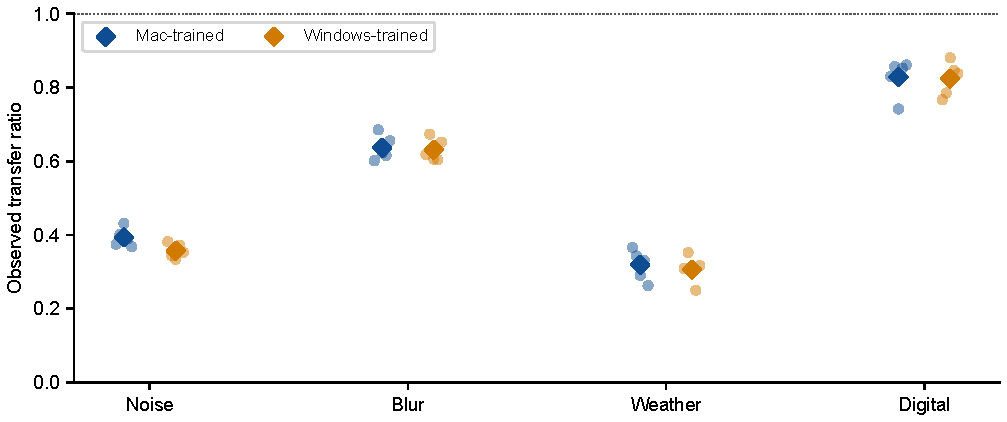
\includegraphics[width=0.86\textwidth]{figures/transfer_ratios.pdf}
\caption{Observed transfer ratios. Diamonds show $\overline D/\overline G$ over five seeds; small points show the five $D_k/G_k$ values. The diamond is not their arithmetic mean. No ratio confidence interval is implied by this display. All eight reference-gain intervals are above zero. Both cohorts use Mac MPS inference.}
\label{fig:ratios}
\end{figure}
\FloatBarrier

\section{Complete held-out-type comparison}
\label{app:types}
\begin{table}[!htbp]
\centering
\small
\setlength{\tabcolsep}{5pt}
\caption{Held-out-type mean gains (pp), averaged equally over five severities within each seed. Intervals summarize five paired seed differences; these are descriptive marginal intervals without multiplicity adjustment.}
\label{tab:types}
\begin{tabular}{lrr}
\toprule
Corruption & Mac $D$ [95\% CI] & Windows $D$ [95\% CI] \\
\midrule
gaussian noise & 18.52 [15.99, 21.05] & 17.44 [16.08, 18.80] \\
shot noise & 17.35 [15.62, 19.08] & 16.21 [14.98, 17.43] \\
impulse noise & 11.74 [10.27, 13.21] & 9.12 [6.50, 11.74] \\
defocus blur & 3.44 [2.73, 4.16] & 3.28 [1.90, 4.66] \\
glass blur & 29.02 [27.04, 31.01] & 29.05 [26.48, 31.62] \\
motion blur & 4.03 [3.27, 4.80] & 3.83 [2.87, 4.79] \\
zoom blur & 7.16 [6.23, 8.10] & 7.38 [5.75, 9.01] \\
snow & 6.20 [5.67, 6.74] & 5.96 [5.37, 6.55] \\
frost & 13.90 [12.74, 15.05] & 13.97 [13.38, 14.57] \\
fog & -7.10 [-7.98, -6.22] & -7.18 [-7.78, -6.57] \\
brightness & -4.28 [-4.80, -3.75] & -4.47 [-4.82, -4.11] \\
contrast & 11.04 [10.23, 11.85] & 11.17 [10.66, 11.67] \\
elastic transform & 4.84 [4.47, 5.20] & 5.26 [4.97, 5.55] \\
pixelate & 8.74 [8.62, 8.86] & 8.60 [6.06, 11.13] \\
jpeg compression & 7.65 [6.35, 8.94] & 8.27 [6.78, 9.75] \\
\bottomrule
\end{tabular}
\end{table}

The accompanying CSVs retain all model/type accuracies and all 75 type--severity cells per model, including negative gains. Figure~\ref{fig:tradeoff} complements main Table~\ref{M-tab:overall} by showing the individual clean/robustness pairs.
\begin{figure}[!htbp]
\centering
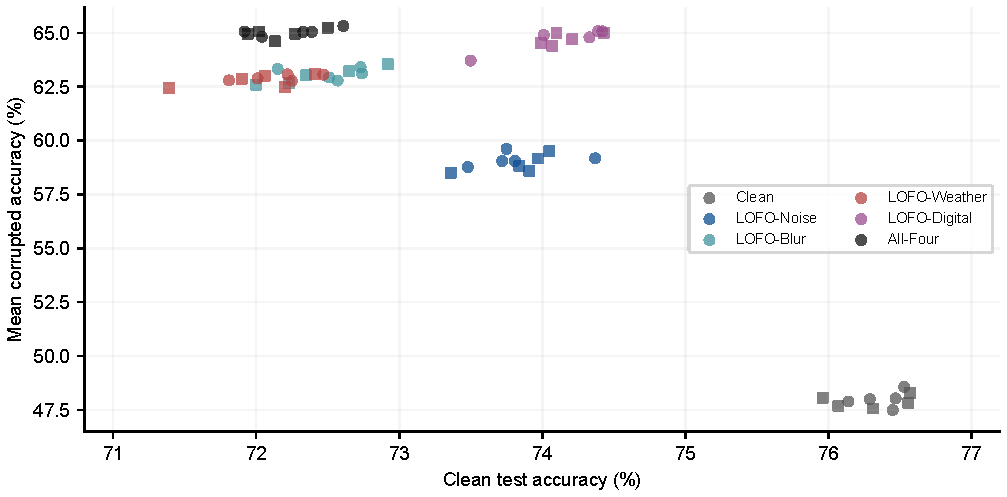
\includegraphics[width=0.83\textwidth]{figures/clean_robustness.pdf}
\caption{Clean versus mean corrupted accuracy. Each point is a trained seed: circles denote Mac training and squares Windows training. Color denotes condition. Axes deliberately show the observed accuracy ranges, with no fitted causal relationship. All 60 points use the same Mac MPS inference pipeline. Source: independently recomputed model scores.}
\label{fig:tradeoff}
\end{figure}
\FloatBarrier

\FloatBarrier
\section{Optimization and environment diagnostics}
\label{app:convergence}
\begin{table}[!htbp]
\centering
\small
\setlength{\tabcolsep}{5pt}
\caption{Selection and late optimization, five seeds per row. Best epochs follow seed order 52,67,999,555,1666. Val100 is mean clean-validation accuracy (\%); $\Delta$ is epoch100 minus epoch91. Losses are cross entropy.}
\label{tab:convergence}
\begin{tabular}{lllr rrr}
\toprule
Training & Condition & Best epochs & Val100 & $\Delta$val pp & $\Delta$train loss & $\Delta$val loss \\
\midrule
Mac & Clean & 97,92,97,93,97 & 76.90 & 0.20 & -0.0006 & -0.0039 \\
Mac & LOFO-Noise & 100,95,100,98,94 & 74.52 & 0.12 & -0.0069 & -0.0090 \\
Mac & LOFO-Blur & 92,96,98,98,99 & 73.20 & 0.17 & -0.0088 & -0.0131 \\
Mac & LOFO-Weather & 98,97,97,98,96 & 72.87 & 0.11 & -0.0052 & -0.0112 \\
Mac & LOFO-Digital & 96,95,87,98,99 & 74.77 & 0.28 & -0.0074 & -0.0145 \\
Mac & All-Four & 96,100,97,98,92 & 72.64 & 0.25 & -0.0092 & -0.0122 \\
Windows & Clean & 94,92,94,95,90 & 77.17 & 0.14 & -0.0006 & -0.0036 \\
Windows & LOFO-Noise & 97,97,96,98,95 & 74.36 & 0.12 & -0.0068 & -0.0118 \\
Windows & LOFO-Blur & 98,99,99,93,100 & 73.16 & 0.28 & -0.0091 & -0.0087 \\
Windows & LOFO-Weather & 92,97,99,91,98 & 72.74 & 0.16 & -0.0050 & -0.0096 \\
Windows & LOFO-Digital & 92,97,93,98,91 & 74.88 & 0.20 & -0.0076 & -0.0108 \\
Windows & All-Four & 96,95,99,98,98 & 72.76 & 0.08 & -0.0085 & -0.0120 \\
\bottomrule
\end{tabular}
\end{table}

\begin{figure}[!htbp]
\centering
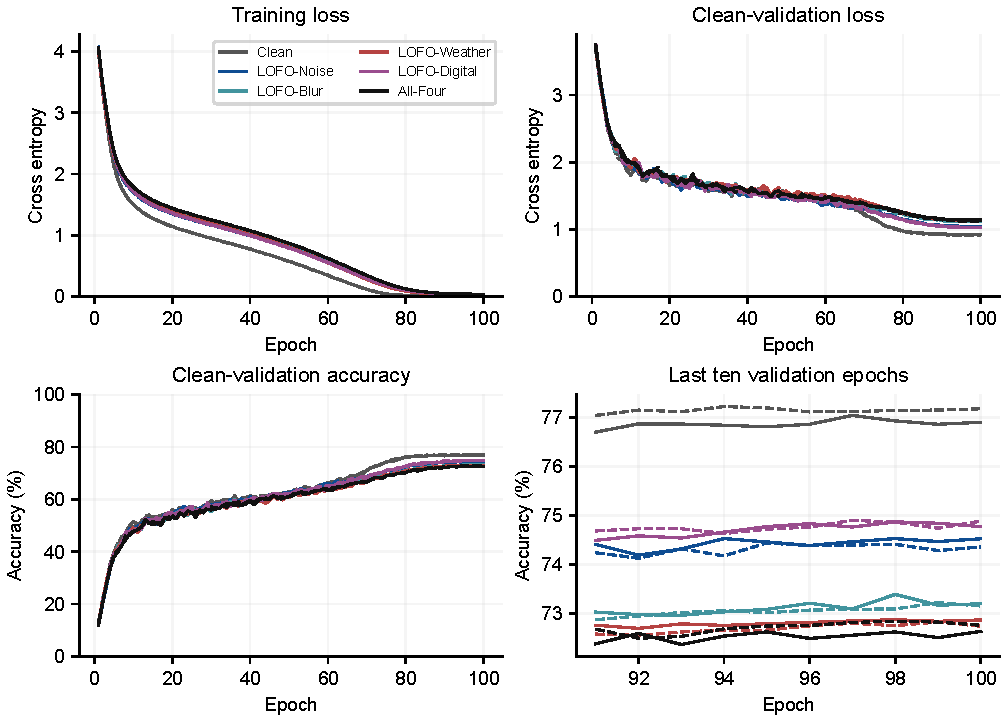
\includegraphics[width=0.98\textwidth]{figures/convergence.pdf}
\caption{Mean training and clean-validation trajectories over five seeds per condition. Solid curves: Mac training; dashed: Windows training. The final panel expands epochs91--100; it is not a separate experiment. All 60 histories contribute. Small late improvements limit claims of complete convergence. Source: original100-epoch history CSVs.}
\label{fig:convergence}
\end{figure}
\label{app:platform}
\begin{figure}[!htbp]
\centering
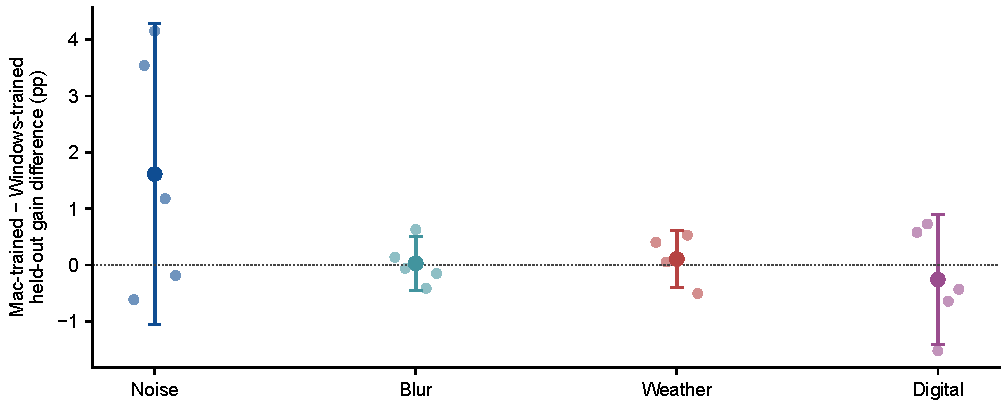
\includegraphics[width=0.85\textwidth]{figures/cross_platform.pdf}
\caption{Matched-seed differences in held-out gain $D$: Mac-trained minus Windows-trained. Small points are five seed differences, with means and nominal95\% $t$ intervals. Intervals including zero do not establish equivalence. Training hardware and dependencies differ, while inference is common Mac MPS.}
\label{fig:platform}
\end{figure}
\FloatBarrier


\FloatBarrier
\section{Operator-policy association matrix}
\label{supp:operator}
\posthoc. For family $F$ and type $c$, define $A_{p,k,F,c}=\overline{\mathrm{Acc}}_{p,k,\mathrm{AllFour},c}-\overline{\mathrm{Acc}}_{p,k,\mathrm{LOFO}_F,c}$, where each bar averages five severities. Reported means, SDs and nominal 95\% $t$ intervals over five training seeds use $t_{0.975,4}$ and paired seed differences. Each policy contrast combines the omitted representative's content with 12.5 percentage points more corruption dose (37.5\% versus 50\%). CSVs contain all seed and cell estimates.
\begin{figure}[!htbp]\centering
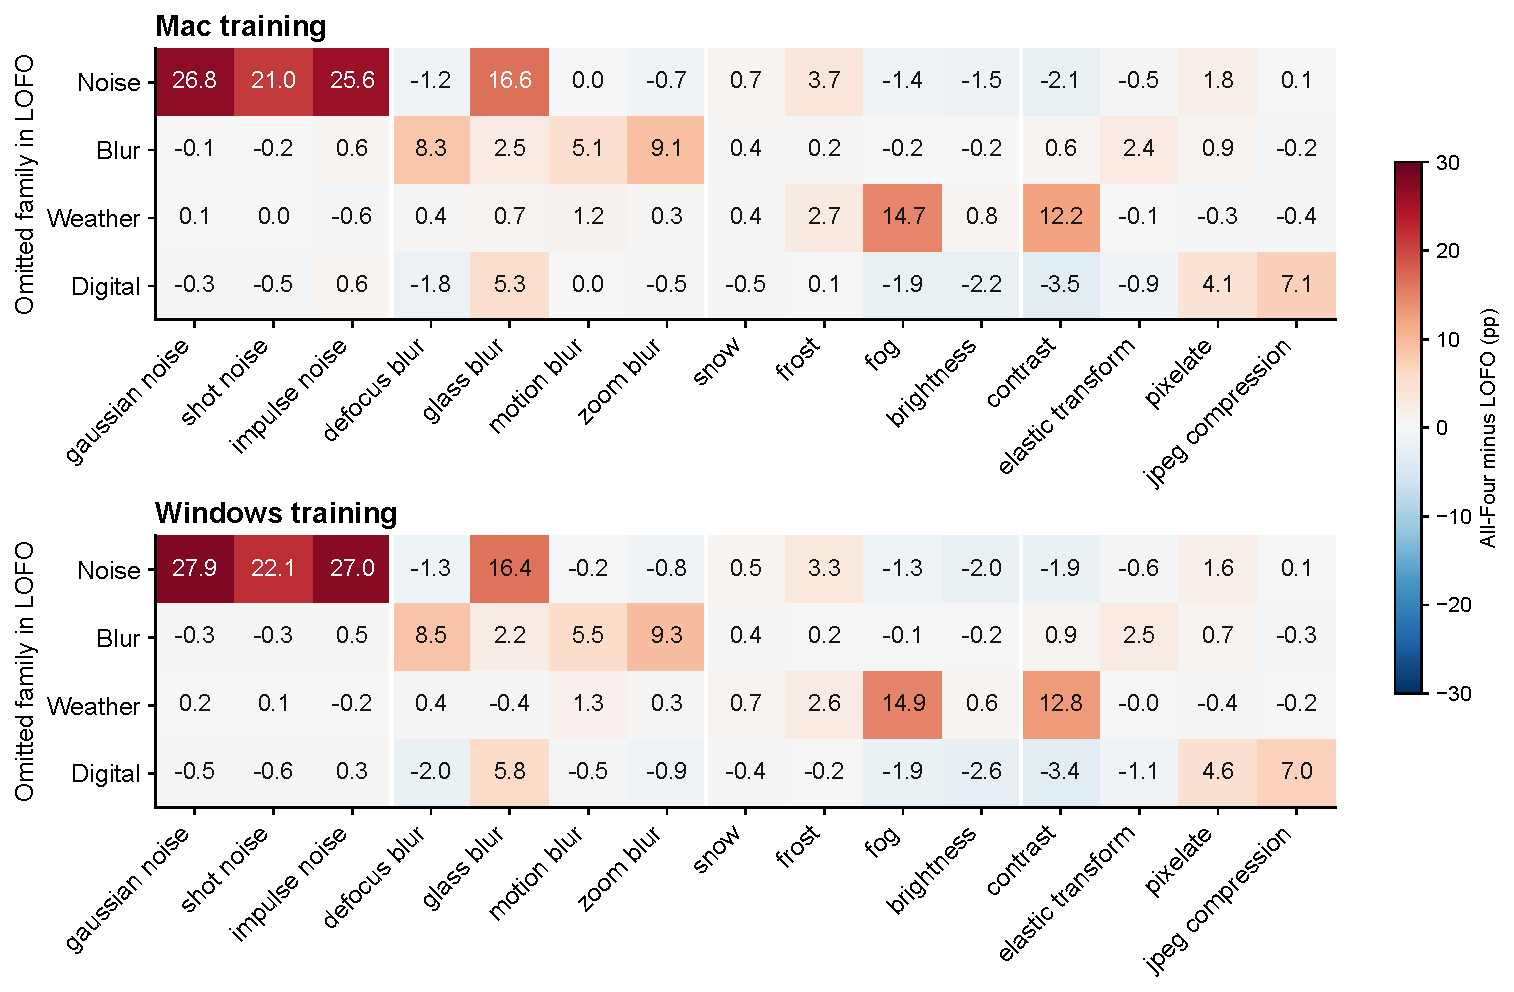
\includegraphics[width=\textwidth]{figures/operator_matrix.pdf}
\caption{Operator association matrices: All-Four minus LOFO, in pp, averaged over severities and then seeds. Rows identify the family omitted in LOFO. Both panels use the same zero-centered scale. Tables~\ref{tab:a1mac} and~\ref{tab:a1win} report SDs and nominal 95\% $t$ intervals over five training seeds. \posthoc.}
\label{fig:operator}\end{figure}
\FloatBarrier
\begingroup\small
\setlength{\tabcolsep}{4pt}
\begin{longtable}{llrrlr}
\caption{Operator association cells, Mac training. Mean and SD are in pp; intervals are nominal 95\% $t$ intervals over five training seeds. BH $q$ values cover the 114 exploratory cells jointly. A dash denotes a designated directional cell tested with H1/H2. \posthoc}\label{tab:a1mac}\\
\toprule
Omitted family & Type & Mean & SD & Interval & BH $q$\\\midrule\endfirsthead
\multicolumn{6}{l}{\tablename\ \thetable{} continued. \posthocshort}\\\toprule
Omitted family & Type & Mean & SD & Interval & BH $q$\\\midrule\endhead
\bottomrule\endfoot
Noise & gaussian noise & 26.83 & 1.14 & [25.42, 28.24] & 1.35e-05\\
Noise & shot noise & 21.01 & 0.79 & [20.03, 21.99] & 1.08e-05\\
Noise & impulse noise & 25.61 & 1.43 & [23.84, 27.38] & --\\
Noise & defocus blur & -1.20 & 0.11 & [-1.34, -1.06] & 0.0001\\
Noise & glass blur & 16.57 & 1.18 & [15.10, 18.04] & --\\
Noise & motion blur & 0.01 & 0.44 & [-0.54, 0.56] & 0.9736\\
Noise & zoom blur & -0.72 & 0.21 & [-0.98, -0.46] & 0.0039\\
Noise & snow & 0.69 & 0.24 & [0.40, 0.98] & 0.0064\\
Noise & frost & 3.73 & 0.21 & [3.46, 4.00] & 3.00e-05\\
Noise & fog & -1.39 & 0.15 & [-1.57, -1.21] & 0.0002\\
Noise & brightness & -1.55 & 0.09 & [-1.66, -1.43] & 3.01e-05\\
Noise & contrast & -2.12 & 0.62 & [-2.89, -1.35] & 0.0039\\
Noise & elastic transform & -0.51 & 0.08 & [-0.61, -0.42] & 0.0005\\
Noise & pixelate & 1.82 & 1.29 & [0.22, 3.41] & 0.0629\\
Noise & jpeg compression & 0.10 & 0.14 & [-0.08, 0.28] & 0.2727\\
Blur & gaussian noise & -0.14 & 0.23 & [-0.42, 0.15] & 0.3337\\
Blur & shot noise & -0.19 & 0.16 & [-0.39, 0.02] & 0.1084\\
Blur & impulse noise & 0.62 & 1.05 & [-0.69, 1.93] & 0.3388\\
Blur & defocus blur & 8.29 & 0.69 & [7.43, 9.16] & 8.78e-05\\
Blur & glass blur & 2.49 & 0.47 & [1.90, 3.08] & 0.0010\\
Blur & motion blur & 5.07 & 0.63 & [4.30, 5.85] & 0.0003\\
Blur & zoom blur & 9.11 & 0.77 & [8.15, 10.07] & 8.78e-05\\
Blur & snow & 0.39 & 0.74 & [-0.52, 1.31] & 0.3710\\
Blur & frost & 0.24 & 0.70 & [-0.63, 1.11] & 0.5382\\
Blur & fog & -0.16 & 0.31 & [-0.54, 0.22] & 0.3710\\
Blur & brightness & -0.23 & 0.34 & [-0.65, 0.19] & 0.2807\\
Blur & contrast & 0.63 & 0.71 & [-0.25, 1.50] & 0.1771\\
Blur & elastic transform & 2.36 & 0.53 & [1.70, 3.01] & 0.0017\\
Blur & pixelate & 0.93 & 0.37 & [0.47, 1.39] & 0.0108\\
Blur & jpeg compression & -0.24 & 0.19 & [-0.48, -0.00] & 0.0872\\
Weather & gaussian noise & 0.11 & 0.22 & [-0.16, 0.38] & 0.3866\\
Weather & shot noise & 0.03 & 0.19 & [-0.21, 0.26] & 0.8132\\
Weather & impulse noise & -0.56 & 0.58 & [-1.28, 0.16] & 0.1490\\
Weather & defocus blur & 0.36 & 0.37 & [-0.10, 0.82] & 0.1490\\
Weather & glass blur & 0.74 & 2.20 & [-1.99, 3.48] & 0.5392\\
Weather & motion blur & 1.16 & 0.63 & [0.39, 1.94] & 0.0279\\
Weather & zoom blur & 0.31 & 0.27 & [-0.02, 0.65] & 0.0997\\
Weather & snow & 0.43 & 0.56 & [-0.27, 1.13] & 0.2359\\
Weather & frost & 2.68 & 0.38 & [2.20, 3.15] & 0.0005\\
Weather & fog & 14.73 & 0.51 & [14.10, 15.37] & 9.93e-06\\
Weather & brightness & 0.75 & 0.35 & [0.32, 1.19] & 0.0177\\
Weather & contrast & 12.18 & 0.56 & [11.49, 12.87] & --\\
Weather & elastic transform & -0.10 & 0.48 & [-0.69, 0.50] & 0.6978\\
Weather & pixelate & -0.33 & 0.37 & [-0.79, 0.13] & 0.1771\\
Weather & jpeg compression & -0.36 & 0.17 & [-0.57, -0.15] & 0.0177\\
Digital & gaussian noise & -0.25 & 0.51 & [-0.88, 0.37] & 0.3866\\
Digital & shot noise & -0.52 & 0.50 & [-1.14, 0.09] & 0.1274\\
Digital & impulse noise & 0.64 & 1.22 & [-0.88, 2.15] & 0.3776\\
Digital & defocus blur & -1.81 & 0.56 & [-2.50, -1.12] & 0.0045\\
Digital & glass blur & 5.34 & 0.91 & [4.22, 6.47] & 0.0008\\
Digital & motion blur & 0.02 & 1.05 & [-1.28, 1.31] & 0.9743\\
Digital & zoom blur & -0.53 & 0.52 & [-1.18, 0.12] & 0.1358\\
Digital & snow & -0.47 & 0.87 & [-1.55, 0.61] & 0.3689\\
Digital & frost & 0.14 & 1.13 & [-1.26, 1.54] & 0.8176\\
Digital & fog & -1.89 & 0.58 & [-2.62, -1.17] & 0.0045\\
Digital & brightness & -2.16 & 0.25 & [-2.46, -1.85] & 0.0002\\
Digital & contrast & -3.49 & 1.01 & [-4.74, -2.23] & 0.0039\\
Digital & elastic transform & -0.93 & 0.61 & [-1.69, -0.18] & 0.0501\\
Digital & pixelate & 4.06 & 0.66 & [3.23, 4.88] & 0.0007\\
Digital & jpeg compression & 7.07 & 0.66 & [6.25, 7.89] & 0.0001\\
\end{longtable}\endgroup

\begingroup\small
\setlength{\tabcolsep}{4pt}
\begin{longtable}{llrrlr}
\caption{Operator association cells, Windows training. Mean and SD are in pp; intervals are nominal 95\% $t$ intervals over five training seeds. BH $q$ values cover the 114 exploratory cells jointly. A dash denotes a designated directional cell tested with H1/H2. \posthoc}\label{tab:a1win}\\
\toprule
Omitted family & Type & Mean & SD & Interval & BH $q$\\\midrule\endfirsthead
\multicolumn{6}{l}{\tablename\ \thetable{} continued. \posthocshort}\\\toprule
Omitted family & Type & Mean & SD & Interval & BH $q$\\\midrule\endhead
\bottomrule\endfoot
Noise & gaussian noise & 27.87 & 0.90 & [26.76, 28.98] & 9.74e-06\\
Noise & shot noise & 22.12 & 0.62 & [21.36, 22.89] & 9.74e-06\\
Noise & impulse noise & 26.98 & 0.96 & [25.79, 28.18] & --\\
Noise & defocus blur & -1.27 & 0.22 & [-1.54, -1.00] & 0.0008\\
Noise & glass blur & 16.36 & 2.16 & [13.69, 19.04] & --\\
Noise & motion blur & -0.21 & 0.58 & [-0.93, 0.50] & 0.5156\\
Noise & zoom blur & -0.84 & 0.13 & [-1.00, -0.68] & 0.0006\\
Noise & snow & 0.54 & 0.26 & [0.22, 0.87] & 0.0197\\
Noise & frost & 3.25 & 0.65 & [2.45, 4.06] & 0.0012\\
Noise & fog & -1.25 & 0.29 & [-1.61, -0.89] & 0.0019\\
Noise & brightness & -1.97 & 0.10 & [-2.09, -1.84] & 2.14e-05\\
Noise & contrast & -1.92 & 0.48 & [-2.51, -1.33] & 0.0025\\
Noise & elastic transform & -0.65 & 0.24 & [-0.94, -0.35] & 0.0078\\
Noise & pixelate & 1.63 & 0.55 & [0.95, 2.32] & 0.0062\\
Noise & jpeg compression & 0.14 & 0.23 & [-0.14, 0.43] & 0.3143\\
Blur & gaussian noise & -0.26 & 0.47 & [-0.84, 0.32] & 0.3646\\
Blur & shot noise & -0.29 & 0.49 & [-0.89, 0.32] & 0.3373\\
Blur & impulse noise & 0.45 & 1.27 & [-1.13, 2.03] & 0.5245\\
Blur & defocus blur & 8.51 & 0.44 & [7.96, 9.05] & 2.14e-05\\
Blur & glass blur & 2.16 & 1.73 & [0.00, 4.31] & 0.0872\\
Blur & motion blur & 5.52 & 0.52 & [4.87, 6.17] & 0.0001\\
Blur & zoom blur & 9.28 & 0.63 & [8.49, 10.07] & 4.95e-05\\
Blur & snow & 0.36 & 0.54 & [-0.32, 1.03] & 0.2949\\
Blur & frost & 0.15 & 0.65 & [-0.65, 0.96] & 0.6725\\
Blur & fog & -0.05 & 0.23 & [-0.34, 0.24] & 0.6808\\
Blur & brightness & -0.21 & 0.28 & [-0.56, 0.13] & 0.2359\\
Blur & contrast & 0.88 & 0.49 & [0.27, 1.49] & 0.0312\\
Blur & elastic transform & 2.45 & 0.43 & [1.92, 2.99] & 0.0008\\
Blur & pixelate & 0.68 & 0.49 & [0.08, 1.29] & 0.0636\\
Blur & jpeg compression & -0.26 & 0.33 & [-0.67, 0.15] & 0.2176\\
Weather & gaussian noise & 0.19 & 0.51 & [-0.44, 0.82] & 0.5156\\
Weather & shot noise & 0.15 & 0.51 & [-0.48, 0.78] & 0.5970\\
Weather & impulse noise & -0.18 & 0.66 & [-1.01, 0.64] & 0.6155\\
Weather & defocus blur & 0.37 & 0.57 & [-0.34, 1.07] & 0.2990\\
Weather & glass blur & -0.40 & 0.95 & [-1.58, 0.79] & 0.4782\\
Weather & motion blur & 1.33 & 0.47 & [0.76, 1.91] & 0.0067\\
Weather & zoom blur & 0.31 & 0.31 & [-0.08, 0.70] & 0.1436\\
Weather & snow & 0.74 & 0.21 & [0.48, 0.99] & 0.0037\\
Weather & frost & 2.56 & 0.31 & [2.17, 2.94] & 0.0003\\
Weather & fog & 14.93 & 0.45 & [14.37, 15.48] & 9.74e-06\\
Weather & brightness & 0.61 & 0.34 & [0.18, 1.03] & 0.0316\\
Weather & contrast & 12.79 & 0.74 & [11.87, 13.71] & --\\
Weather & elastic transform & -0.03 & 0.51 & [-0.66, 0.60] & 0.9226\\
Weather & pixelate & -0.36 & 0.38 & [-0.84, 0.11] & 0.1490\\
Weather & jpeg compression & -0.16 & 0.42 & [-0.68, 0.35] & 0.5004\\
Digital & gaussian noise & -0.48 & 0.14 & [-0.66, -0.31] & 0.0039\\
Digital & shot noise & -0.63 & 0.13 & [-0.79, -0.47] & 0.0012\\
Digital & impulse noise & 0.35 & 0.88 & [-0.74, 1.44] & 0.4948\\
Digital & defocus blur & -2.02 & 0.37 & [-2.48, -1.56] & 0.0009\\
Digital & glass blur & 5.79 & 1.69 & [3.69, 7.89] & 0.0039\\
Digital & motion blur & -0.46 & 0.43 & [-1.00, 0.08] & 0.1271\\
Digital & zoom blur & -0.93 & 0.19 & [-1.17, -0.70] & 0.0012\\
Digital & snow & -0.37 & 0.34 & [-0.79, 0.05] & 0.1203\\
Digital & frost & -0.23 & 0.45 & [-0.79, 0.34] & 0.3866\\
Digital & fog & -1.89 & 0.14 & [-2.07, -1.72] & 6.49e-05\\
Digital & brightness & -2.58 & 0.44 & [-3.13, -2.03] & 0.0008\\
Digital & contrast & -3.37 & 0.28 & [-3.72, -3.02] & 8.78e-05\\
Digital & elastic transform & -1.14 & 0.34 & [-1.56, -0.72] & 0.0039\\
Digital & pixelate & 4.59 & 1.18 & [3.12, 6.06] & 0.0028\\
Digital & jpeg compression & 7.03 & 0.30 & [6.65, 7.41] & 1.35e-05\\
\end{longtable}\endgroup

\subsection{Directional hypotheses and exploratory multiplicity}
H1 requires positive Weather/contrast policy differences in both platforms. H2 requires positive Noise/impulse-noise and Noise/glass-blur differences in both platforms. H3 requires negative brightness gains relative to Clean in every augmented condition in both platforms. For each claim the largest component one-sided paired $t$ probability is the intersection--union probability. Holm adjusts only the three conjunctions. All component directions agree in the observed seed values; the hypotheses concern mean differences. Remaining matrix cells form a single exploratory BH family of 114 cells; designated H1/H2 cells are excluded. The claims retain their post-hoc exploratory status after adjustment.
\begingroup\small
\setlength{\tabcolsep}{4pt}
\begin{longtable}{llllrlr}
\caption{Directional components. H1/H2 compare All-Four with the named LOFO; H3 compares the augmented condition with Clean. Means are pp; each interval is a nominal 95\% $t$ interval over five training seeds. One-sided tests follow the frozen directions. \posthoc}\label{tab:hcomponents}\\
\toprule
Claim & Platform & Contrast & Type & Mean & Interval & $p$\\\midrule\endfirsthead
\multicolumn{7}{l}{\tablename\ \thetable{} continued. \posthocshort}\\\toprule
Claim & Platform & Contrast & Type & Mean & Interval & $p$\\\midrule\endhead
\bottomrule\endfoot
H1 & Mac & weather & contrast & 12.18 & [11.49, 12.87] & 5.21e-07\\
H2 & Mac & noise & impulse noise & 25.61 & [23.84, 27.38] & 1.15e-06\\
H2 & Mac & noise & glass blur & 16.57 & [15.10, 18.04] & 3.11e-06\\
H3 & Mac & LOFO-noise & brightness & -1.98 & [-2.42, -1.53] & 0.0001\\
H3 & Mac & LOFO-blur & brightness & -3.30 & [-3.70, -2.89] & 1.15e-05\\
H3 & Mac & LOFO-weather & brightness & -4.28 & [-4.80, -3.75] & 1.11e-05\\
H3 & Mac & LOFO-digital & brightness & -1.37 & [-1.81, -0.92] & 0.0005\\
H3 & Mac & all four & brightness & -3.53 & [-3.92, -3.13] & 7.75e-06\\
H1 & Windows & weather & contrast & 12.79 & [11.87, 13.71] & 1.37e-06\\
H2 & Windows & noise & impulse noise & 26.98 & [25.79, 28.18] & 1.93e-07\\
H2 & Windows & noise & glass blur & 16.36 & [13.69, 19.04] & 3.53e-05\\
H3 & Windows & LOFO-noise & brightness & -1.89 & [-2.28, -1.50] & 8.94e-05\\
H3 & Windows & LOFO-blur & brightness & -3.65 & [-4.02, -3.28] & 5.46e-06\\
H3 & Windows & LOFO-weather & brightness & -4.47 & [-4.82, -4.11] & 1.99e-06\\
H3 & Windows & LOFO-digital & brightness & -1.28 & [-1.65, -0.91] & 0.0003\\
H3 & Windows & all four & brightness & -3.86 & [-4.29, -3.43] & 8.00e-06\\
\end{longtable}\endgroup

\begingroup\small
\setlength{\tabcolsep}{4pt}
\begin{longtable}{lrrr}
\caption{Three conjunction claims across both environments: H1 (fog slot/contrast); H2 (Gaussian slot/impulse noise and glass blur); H3 (brightness loss in every augmented condition). The largest component probability defines each conjunction; Holm adjusts only these three claims. \posthoc}\label{tab:holm}\\
\toprule
Claim & Components & Conjunction $p$ & Holm $p$\\\midrule\endfirsthead
\multicolumn{4}{l}{\tablename\ \thetable{} continued. \posthocshort}\\\toprule
Claim & Components & Conjunction $p$ & Holm $p$\\\midrule\endhead
\bottomrule\endfoot
H1 & 2 & 1.37e-06 & 4.11e-06\\
H2 & 4 & 3.53e-05 & 7.06e-05\\
H3 & 10 & 0.0005 & 0.0005\\
\end{longtable}\endgroup

\FloatBarrier
\section{Transfer groups and clean-accuracy costs}
\label{supp:groups}
\posthoc. Within each LOFO condition, the three disjoint groups partition all 15 types: (a) the three training representatives, (b) the held-out family, and (c) untrained types in represented families. Each seed's gain averages type-level LOFO-minus-Clean differences equally. Group sizes differ; types are not independent training repetitions. Group (c) means are positive in all platform/LOFO combinations. Negative held-out fog and brightness gains and heterogeneous policy contrasts remain visible. Regularization remains a plausible explanation for these observations.
\begingroup\small
\setlength{\tabcolsep}{4pt}
\begin{longtable}{lllrrl}
\caption{Paired LOFO gains over Clean by group: (a) three retained representatives; (b) held-out family; (c) untrained types in represented families. Equal type weighting within each group; nominal 95\% $t$ interval over five training seeds. Units: pp. \posthoc}\label{tab:groups}\\
\toprule
Platform & Held out & Group & Mean & SD & Interval\\\midrule\endfirsthead
\multicolumn{6}{l}{\tablename\ \thetable{} continued. \posthocshort}\\\toprule
Platform & Held out & Group & Mean & SD & Interval\\\midrule\endhead
\bottomrule\endfoot
Mac & Noise & a & 12.19 & 0.49 & [11.59, 12.80]\\
Mac & Noise & b & 15.87 & 1.14 & [14.45, 17.28]\\
Mac & Noise & c & 9.21 & 0.49 & [8.60, 9.82]\\
Mac & Blur & a & 22.75 & 0.91 & [21.61, 23.88]\\
Mac & Blur & b & 10.92 & 0.69 & [10.06, 11.77]\\
Mac & Blur & c & 14.36 & 0.28 & [14.01, 14.72]\\
Mac & Weather & a & 23.90 & 0.90 & [22.78, 25.02]\\
Mac & Weather & b & 2.18 & 0.37 & [1.72, 2.64]\\
Mac & Weather & c & 17.93 & 0.46 & [17.36, 18.49]\\
Mac & Digital & a & 22.89 & 0.83 & [21.86, 23.92]\\
Mac & Digital & b & 8.07 & 0.48 & [7.47, 8.67]\\
Mac & Digital & c & 18.73 & 0.67 & [17.90, 19.56]\\
Windows & Noise & a & 12.40 & 0.58 & [11.69, 13.12]\\
Windows & Noise & b & 14.25 & 1.17 & [12.81, 15.70]\\
Windows & Noise & c & 9.50 & 0.65 & [8.69, 10.30]\\
Windows & Blur & a & 22.98 & 0.42 & [22.45, 23.50]\\
Windows & Blur & b & 10.89 & 0.84 & [9.84, 11.93]\\
Windows & Blur & c & 14.30 & 0.29 & [13.95, 14.66]\\
Windows & Weather & a & 24.00 & 0.61 & [23.24, 24.76]\\
Windows & Weather & b & 2.07 & 0.27 & [1.73, 2.41]\\
Windows & Weather & c & 17.89 & 0.27 & [17.56, 18.23]\\
Windows & Digital & a & 23.08 & 0.38 & [22.61, 23.55]\\
Windows & Digital & b & 8.32 & 0.75 & [7.40, 9.25]\\
Windows & Digital & c & 18.76 & 0.32 & [18.36, 19.16]\\
\end{longtable}\endgroup

\begin{figure}[!htbp]\centering
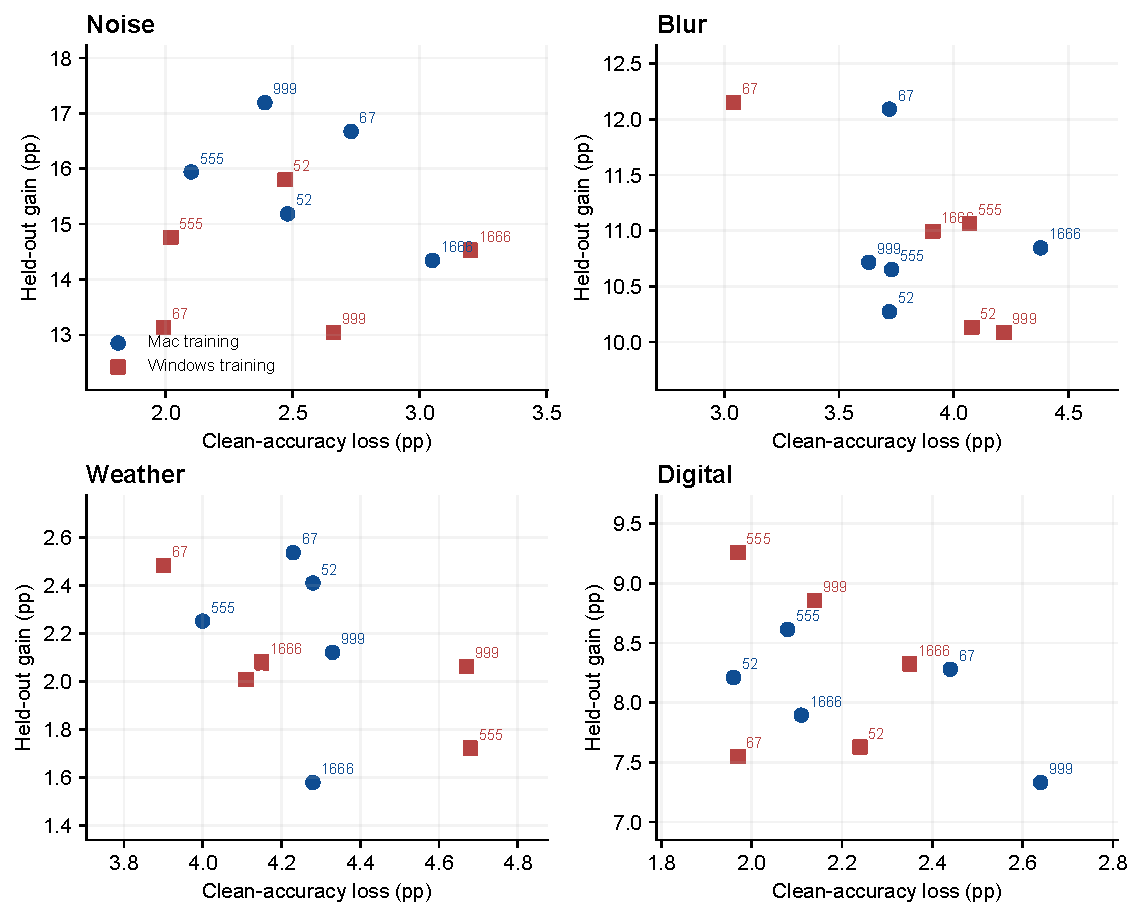
\includegraphics[width=.93\textwidth]{figures/clean_loss_heldout_gain.pdf}
\caption{Per-seed clean-accuracy loss versus held-out-family gain. Positive horizontal values indicate less clean accuracy than matched Clean. Seed identifiers label points; shape and color indicate training environment. No regression or causal interpretation is fitted. Source: A2\_group\_seed.csv, group (b). \posthoc.}
\label{fig:lossscatter}\end{figure}
\FloatBarrier
\begin{figure}[!htbp]\centering
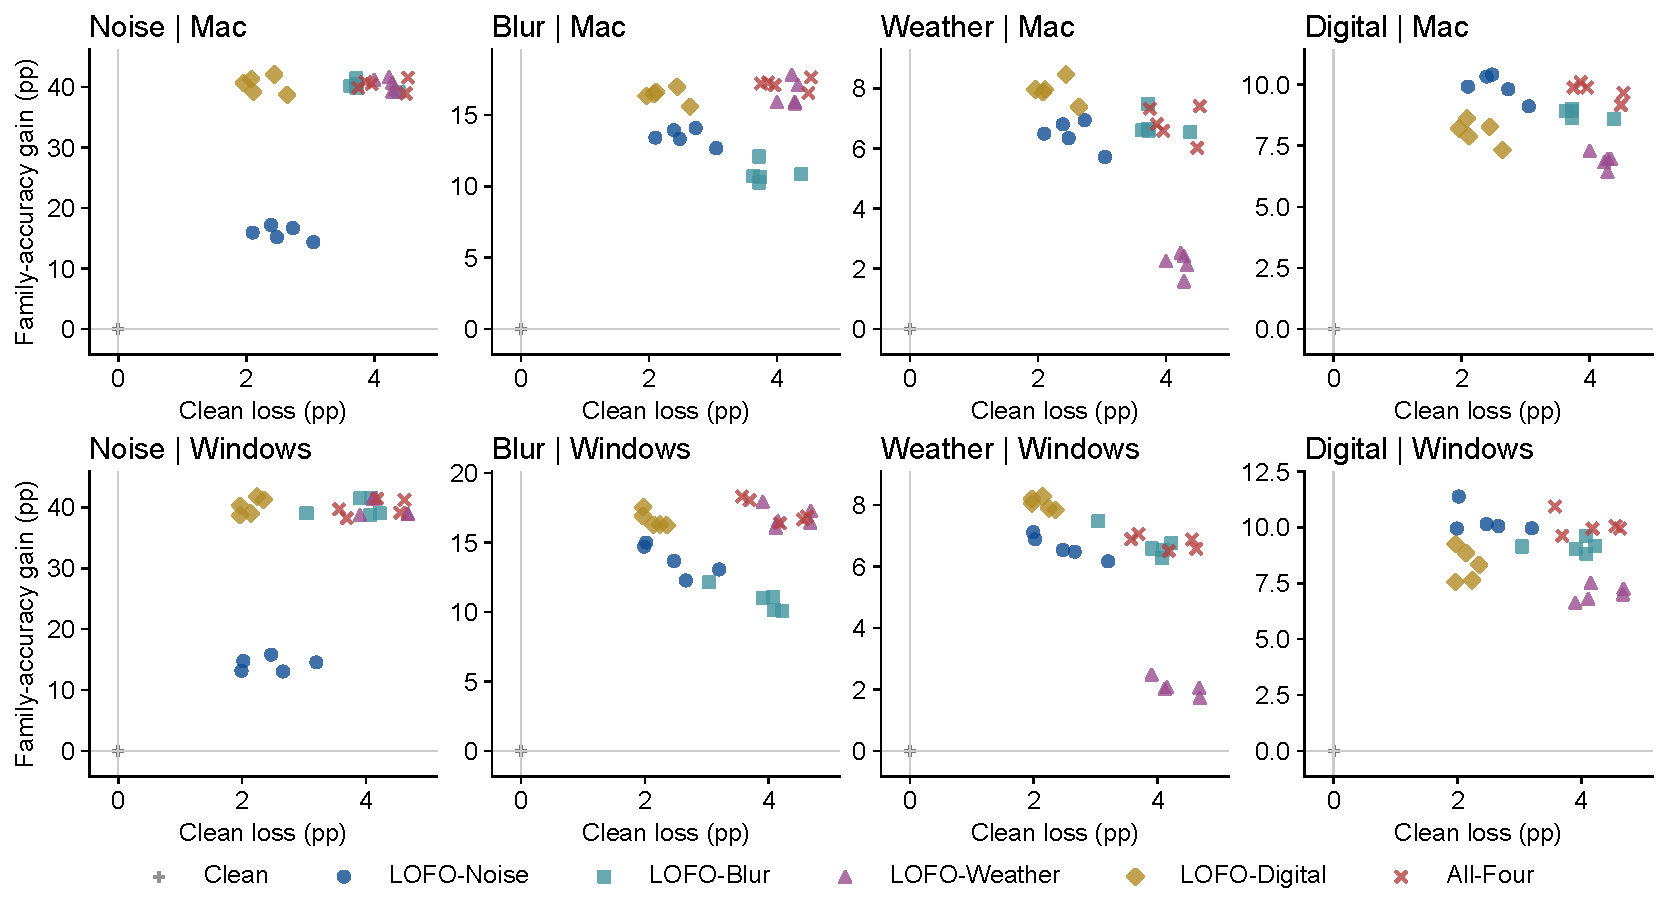
\includegraphics[width=\textwidth]{figures/all_condition_clean_family_scatter.pdf}
\caption{Clean-accuracy loss versus family-accuracy gain for all six conditions and all five seeds, separately for each training environment and family. The five Clean points coincide at the origin. Only LOFO for the panel's named family holds that family out; other policies may train on its representative. This display therefore labels family gains rather than calling every point held-out transfer. No regression or mechanism is inferred. Source: all\_condition\_clean\_family\_scatter.csv. Post-hoc exploratory; \posthoc.}
\label{fig:allscatter}\end{figure}
\FloatBarrier
\section{Matched-seed platform equivalence}
\label{supp:equivalence}
\posthoc. Differences are computed for each matched seed: \[z_{k,F}=D_{\mathrm{Mac},k,F}-D_{\mathrm{Windows},k,F}.\] TOST compares their mean with fixed bounds $\pm\delta$ using df=4, with primary $\delta=1.0$ pp and sensitivity $\delta=0.5$ pp. Both one-sided probabilities must be below 0.05, equivalent to the 90\% interval lying strictly within the bounds. The 95\% interval estimates the mean difference; TOST separately assesses equivalence. Blur and Weather meet both margins; Noise and Digital do not. Power is low with five matched seeds, so a negative TOST decision is inconclusive. These exploratory decisions apply to individual families. Hardware and software differ together, and inference uses a common backend; hardware-only effects and inference portability require separate evaluation.
\begingroup\small
\setlength{\tabcolsep}{4pt}
\begin{longtable}{lrrrlrl}
\caption{Matched-seed Mac-minus-Windows $D$. TOST uses df=4, one-sided alpha=0.05, primary margin 1.0 pp and sensitivity margin 0.5 pp. The 90\% interval is the TOST interval; the nominal 95\% $t$ interval over five training seeds is supplied in the CSV. Decisions are exploratory and family-specific, with no simultaneous equivalence guarantee. \posthoc}\label{tab:tost}\\
\toprule
Family & Margin & Mean & SD & 90\% interval & $p_{\rm TOST}$ & Supported\\\midrule\endfirsthead
\multicolumn{7}{l}{\tablename\ \thetable{} continued. \posthocshort}\\\toprule
Family & Margin & Mean & SD & 90\% interval & $p_{\rm TOST}$ & Supported\\\midrule\endhead
\bottomrule\endfoot
Noise & 1.0 & 1.61 & 2.15 & [-0.44, 3.67] & 0.7209 & No\\
Noise & 0.5 & 1.61 & 2.15 & [-0.44, 3.67] & 0.8442 & No\\
Blur & 1.0 & 0.03 & 0.39 & [-0.34, 0.40] & 0.0026 & Yes\\
Blur & 0.5 & 0.03 & 0.39 & [-0.34, 0.40] & 0.0271 & Yes\\
Weather & 1.0 & 0.11 & 0.40 & [-0.27, 0.49] & 0.0038 & Yes\\
Weather & 0.5 & 0.11 & 0.40 & [-0.27, 0.49] & 0.0473 & Yes\\
Digital & 1.0 & -0.26 & 0.93 & [-1.14, 0.63] & 0.0742 & No\\
Digital & 0.5 & -0.26 & 0.93 & [-1.14, 0.63] & 0.2949 & No\\
\end{longtable}\endgroup

\paragraph{Independent numerical verification.}
Post-hoc exploratory equivalence analysis, specified before computation of the additional statistics, not confirmatory. We independently reconstruct $D$ from saved type accuracies, average types within each seed, and form $z_k=D_{\mathrm{Mac},k}-D_{\mathrm{Windows},k}$. For $n=5$ and df=4, $p_L=1-F_{t_4}((\bar z+\delta)/\mathrm{SE})$, $p_U=F_{t_4}((\bar z-\delta)/\mathrm{SE})$, and $p_{\mathrm{TOST}}=\max(p_L,p_U)$. Equivalence requires both one-sided probabilities below 0.05, or the unrounded 90\% interval strictly inside $(-\delta,\delta)$. Equivalence therefore rests on the stated margin and both one-sided tests. Table~\ref{tab:tostverify} gives both probabilities at both margins; Table~\ref{tab:tostseeds} retains the five matched differences. All original A3 statistics agree within $10^{-11}$. Weather's sensitivity-margin decision is close to the boundary and is based on unrounded values. Low power and uncertain paired normality with five seeds limit interpretation; software and hardware differ together.
\begin{table}[!htbp]
\centering\small
\setlength{\tabcolsep}{4pt}
\caption{Independent matched-seed TOST check. Means, SDs and intervals are pp; $n=5$, df=4. Decisions use unrounded probabilities. Post-hoc exploratory; not confirmatory.}\label{tab:tostverify}
\begin{tabular}{lrrrlrr}\toprule
Family & $\delta$ & Mean & SD & 90\% interval & $p_L$ & $p_U$\\\midrule
Noise & 1.0 & 1.6141 & 2.1528 & [-0.438338, 3.666604] & 0.026624 & 0.720882\\
Noise & 0.5 & 1.6141 & 2.1528 & [-0.438338, 3.666604] & 0.046539 & 0.844210\\
Blur & 1.0 & 0.0301 & 0.3896 & [-0.341330, 0.401530] & 0.002049 & 0.002550\\
Blur & 0.5 & 0.0301 & 0.3896 & [-0.341330, 0.401530] & 0.019153 & 0.027131\\
Weather & 1.0 & 0.1084 & 0.4013 & [-0.274166, 0.490966] & 0.001745 & 0.003830\\
Weather & 0.5 & 0.1084 & 0.4013 & [-0.274166, 0.490966] & 0.013761 & 0.047257\\
Digital & 1.0 & -0.2567 & 0.9298 & [-1.143158, 0.629758] & 0.074185 & 0.019539\\
Digital & 0.5 & -0.2567 & 0.9298 & [-1.143158, 0.629758] & 0.294944 & 0.071456\\
\bottomrule\end{tabular}
\end{table}

\begin{table}[!htbp]
\centering\small
\setlength{\tabcolsep}{4pt}
\caption{Mac-minus-Windows differences in LOFO-minus-Clean held-out-family gain, in pp. Columns are matched seed identifiers. Post-hoc exploratory; not confirmatory.}\label{tab:tostseeds}
\begin{tabular}{lrrrrr}\toprule
Family & 52 & 67 & 999 & 555 & 1666\\\midrule
Noise & -0.614667 & 3.540667 & 4.150667 & 1.178667 & -0.184667\\
Blur & 0.139000 & -0.058000 & 0.630000 & -0.412500 & -0.148000\\
Weather & 0.402500 & 0.053500 & 0.059500 & 0.530000 & -0.503500\\
Digital & 0.582500 & 0.729000 & -1.523000 & -0.642500 & -0.429500\\
\bottomrule\end{tabular}
\end{table}


\section{Variance structure}
\label{supp:variance}
\posthoc. $D$ is LOFO-minus-Clean and $G$ is All-Four-minus-Clean on the named family. The platform shift divided by within-platform RMS seed SD expresses the shift relative to seed variation. It is a descriptive scale summary; variance components would require a separate model. Only two training environments are observed, with hardware and dependencies confounded; both use common Mac MPS inference.
\begin{table}[!htbp]\centering\small
\setlength{\tabcolsep}{4pt}
\caption{Variance structure for $D$ and $G$. SDs are between seeds within each environment. Shift is Mac minus Windows; RMS SD is the square root of the mean of the two squared SDs. The signed ratio is shift divided by RMS SD; it is descriptive and does not pool ten seeds. All columns except the ratio are pp. \posthoc}\label{tab:variance}
\begin{tabular}{llrrrrr}
\toprule
Family & Measure & Mac SD & Win SD & Shift & RMS SD & Shift/SD\\\midrule
Noise & D & 1.140 & 1.167 & 1.614 & 1.154 & 1.399\\
Noise & G & 0.989 & 1.379 & 0.439 & 1.200 & 0.366\\
Blur & D & 0.691 & 0.843 & 0.030 & 0.771 & 0.039\\
Blur & G & 0.402 & 0.863 & -0.096 & 0.673 & -0.142\\
Weather & D & 0.372 & 0.272 & 0.108 & 0.326 & 0.333\\
Weather & G & 0.567 & 0.234 & 0.050 & 0.433 & 0.115\\
Digital & D & 0.483 & 0.747 & -0.257 & 0.629 & -0.408\\
Digital & G & 0.357 & 0.494 & -0.357 & 0.431 & -0.828\\
\bottomrule\end{tabular}\end{table}

\section{Addendum sensitivity}
\label{supp:sensitivity}
\posthoc. Deleting one seed at a time changes the A1 cell mean by at most 0.776100 pp. The largest absolute change in $T=\overline D/\overline G$ is 0.021969; all retained reference means are positive. Excluding the ten previously identified exact-overlap identities, leaving 9,990 images, changes an A1 cell mean by at most 0.016142 pp and an individual seed cell by at most 0.025241 pp. Official results are unchanged. The complete deletion and overlap tables retain every cell; near-duplicate and validation-selection effects remain possible.
\begingroup\small
\setlength{\tabcolsep}{4pt}
\begin{longtable}{llrl}
\caption{Maximum absolute sensitivity changes. LOO deletes one training seed at a time; overlap deletion removes the same ten test identities from each setting. T changes are dimensionless; A1 changes are pp. Full cell and seed deletions are supplied as CSVs. \posthoc}\label{tab:sensitivity}\\
\toprule
Platform & Analysis & Maximum & Units\\\midrule\endfirsthead
\multicolumn{4}{l}{\tablename\ \thetable{} continued. \posthocshort}\\\toprule
Platform & Analysis & Maximum & Units\\\midrule\endhead
\bottomrule\endfoot
Mac & A1 LOO mean & 0.683000 & pp\\
Mac & A1 overlap mean & 0.012438 & pp\\
Mac & A1 overlap seed & 0.018875 & pp\\
Mac & T LOO & 0.021969 & ratio\\
Windows & A1 LOO mean & 0.776100 & pp\\
Windows & A1 overlap mean & 0.016142 & pp\\
Windows & A1 overlap seed & 0.025241 & pp\\
Windows & T LOO & 0.014199 & ratio\\
Across platforms & A1 LOO mean & 0.776100 & pp\\
Across platforms & A1 overlap mean & 0.016142 & pp\\
Across platforms & A1 overlap seed & 0.025241 & pp\\
Across platforms & T LOO & 0.021969 & ratio\\
\end{longtable}\endgroup

\section{Additional original figures and implementation detail}
\label{supp:implementation}
This section contains the original figures and implementation details moved from the main manuscript.
\begin{figure}[!htbp]
\centering
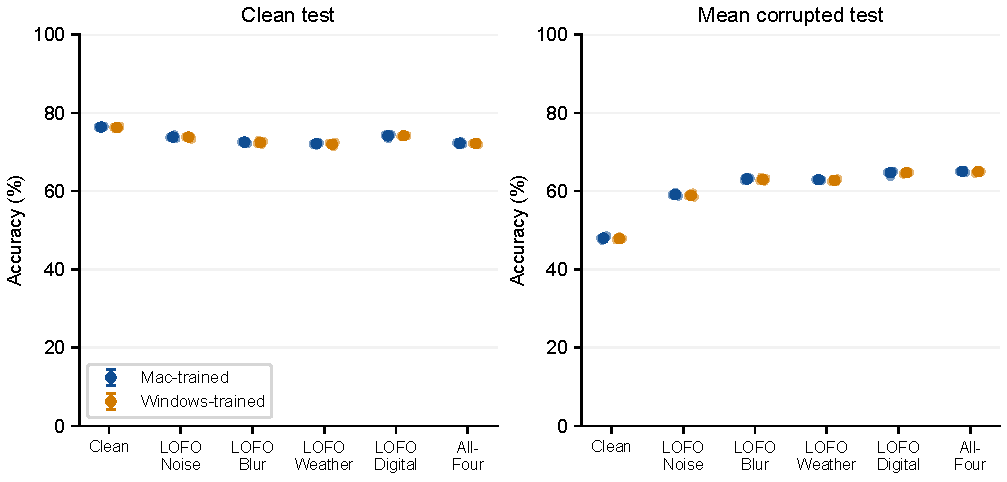
\includegraphics[width=\textwidth]{figures/overall_accuracy.pdf}
\caption{Overall test accuracy by condition and training environment. Small points are five seed results per condition; larger points and bars show means and nominal 95\% $t$ intervals. Corrupted accuracy averages 75 cells within each seed. Both cohorts use Mac MPS inference. Axes start at zero. Source: independently recounted per-condition predictions.}
\label{fig:overall}
\end{figure}
\begin{figure}[!htbp]
\centering
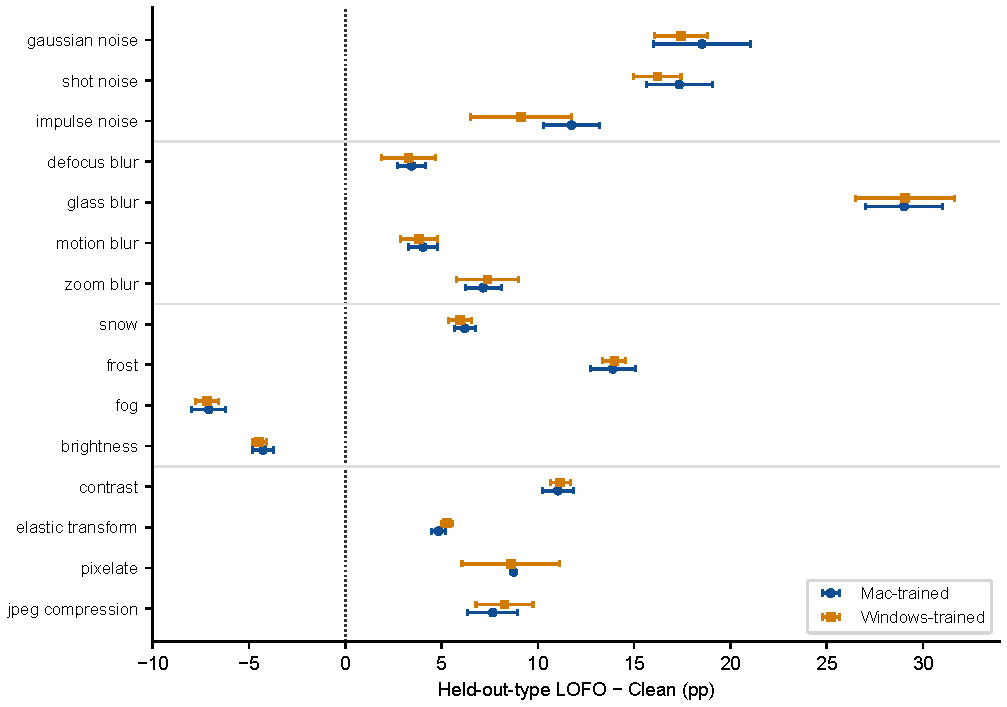
\includegraphics[width=0.96\textwidth]{figures/type_heterogeneity.pdf}
\caption{Held-out-type gains over Clean, averaged over five severities within each seed. Points and bars show means and nominal 95\% $t$ intervals for five paired seed differences. Each type uses the model excluding its family; horizontal separators mark Noise, Blur, Weather and Digital. All types are shown, including negative fog and brightness results. These marginal intervals are descriptive, not multiplicity-adjusted tests.}
\label{fig:types}
\end{figure}
\begin{figure}[!htbp]
\centering
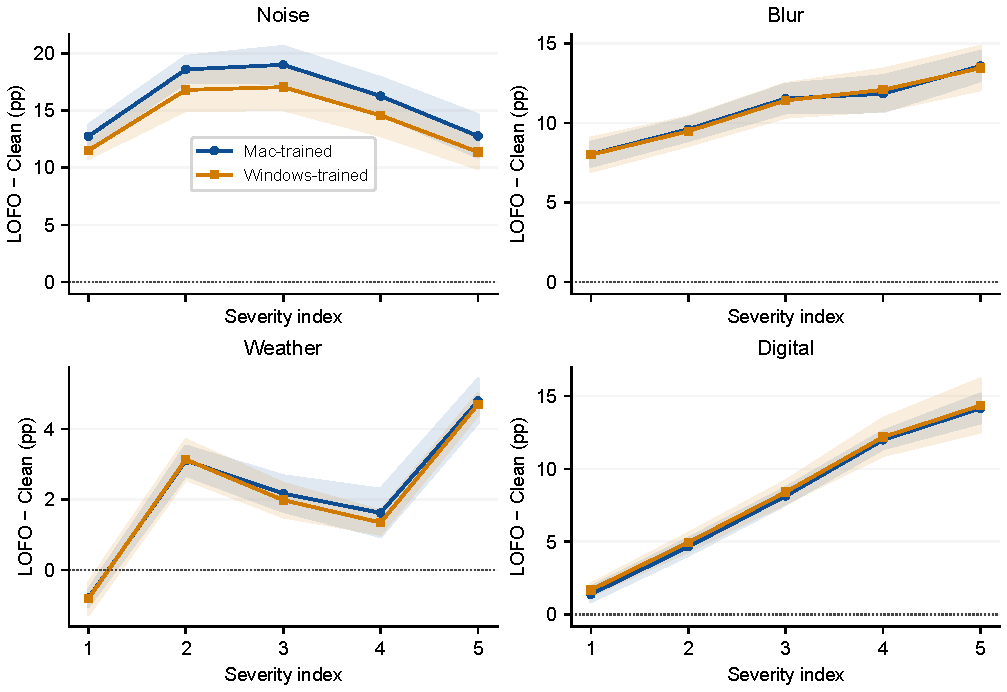
\includegraphics[width=0.94\textwidth]{figures/severity_gains.pdf}
\caption{Excluded-family LOFO$-$Clean gains by severity. Each seed first averages member corruption types; curves and shaded bands show the mean and nominal 95\% $t$ interval over five paired seeds. Zero marks no gain. Severity indices do not define a common physical scale across corruption types. Source: all held-out type--severity cells, without selection of favorable levels.}
\label{fig:severity}
\end{figure}
\FloatBarrier
The random streams are keyed by training seed, epoch and original image index. Separate BLAKE2b-derived 32-bit seeds control spatial choices, branch selection, severity, operator parameters and minibatch order. The condition is absent from these keys, so retained operator choices and pixels match across conditions for the same presentation. The operator name additionally keys its parameter stream. Across all saved epochs, operator-by-severity counts match exactly in every condition retaining the operator, and the count histories match between training platforms for each seed. Independent regeneration of two complete seed-52 exposure epochs and sampled transform checks support the implementation; counts alone do not reconstruct every training pixel.

We adapt the CIFAR-specific reference code~\cite{cifarreference} and give each operator an explicit random generator. We clip and truncate its output to unsigned 8-bit RGB before tensor conversion. Appendix~\ref{app:records} gives the source identity and severity settings. Shared-operator matching fixes retained-operator frequencies while preserving the difference in total corruption rates.


We train for 100 epochs with batch size 128 and stochastic gradient descent: initial learning rate 0.1, momentum 0.9, and weight decay $5\times10^{-4}$. We disable Nesterov momentum, automatic mixed precision (AMP) and label smoothing. Cosine annealing uses $T_{\max}=100$ and $\eta_{\min}=0$, stepped at epoch end. Each epoch consumes all fitting images, retaining the last partial batch, for 352 updates and 35,200 updates per run. After augmentation, we normalize FP32 RGB values in $[0,1]$ with mean $(0.5071,0.4867,0.4408)$ and standard deviation $(0.2675,0.2565,0.2761)$. Clean validation uses only tensor conversion and normalization. We minimize cross-entropy and select the first epoch with the highest clean-validation accuracy, using a strict-improvement rule.

Python, NumPy and PyTorch generators are seeded. Deterministic algorithms are requested, cuDNN benchmarking and TensorFloat-32 are disabled, and epoch IDs are passed explicitly to two persistent data-loader workers. Saved checkpoints contain optimizer, scheduler and RNG states for resumption. These controls standardize the training procedure across heterogeneous backends and library versions; bitwise reproducibility remains unverified.


For model condition $m$, corruption $c$, severity $s$, and $n=10{,}000$ identities, percentage accuracy is
\begin{equation}
A_{m,c,s}=\frac{100}{n}\sum_{i=1}^{n}\mathbf{1}\{f_m(x_i^{c,s})=y_i\}.
\end{equation}
Platform and training-seed indices are suppressed in this equation. Family accuracy and overall corrupted accuracy are
\begin{equation}
A_{m,F}=\frac{1}{5|\mathcal{C}_F|}\sum_{c\in\mathcal{C}_F}\sum_{s=1}^{5}A_{m,c,s},\qquad
A_{m,\mathcal C}=\frac1{75}\sum_{F\in\mathcal F}\sum_{c\in\mathcal C_F}\sum_{s=1}^{5}A_{m,c,s}.
\end{equation}
We weight corruption types and severities equally: Noise contributes $3/15$ and each other family $4/15$ to overall corrupted accuracy. We report clean accuracy separately. The error $100-A_{m,\mathcal C}$ is unnormalized; mean corruption error (mCE) additionally normalizes errors against a reference model.


\subsection{Original cohort and protocol account}
\paragraph{Training cohorts and common evaluation.}
\label{supp:cohortrecord}
The replication contains $6\times5\times2=60$ completed training runs. Mac training uses MPS with PyTorch 2.15.0 and torchvision 0.29.2; Windows training uses an RTX 3050 Ti Laptop GPU with PyTorch 2.14.1+cu130 and torchvision 0.29.1+cu130. Both use FP32, identical frozen source, split, initialization files and augmentation schedules. Python versions also differ, as recorded in Appendix~\ref{app:records}. The replications compare training environments with joint differences in hardware and software.

Both sets of selected checkpoints were evaluated on Mac MPS with FP32, batch size 128, fixed normalization and model evaluation mode. We used no resizing, test-time augmentation, calibration, adaptation or checkpoint reselection. Each cohort's evaluation was gated on completion of all 30 training runs. Fifteen corruption types at five severities plus clean give 76 settings per checkpoint and 4,560 model--setting combinations. Every setting evaluates 10,000 predictions against official labels. Recounting all 45.6 million cached decisions reproduces every saved correct count. The training-platform label in a result file does not denote its inference platform.

\paragraph{Frozen protocol and independent checks.}
\label{supp:protocolrecord}
The original seed-42 outcomes were exploratory and informed the study design. The v3 training source, split, initializations and operator references were frozen before production training. A separate analysis protocol was accepted on 8 November 2026 at 13:41:38 UTC, before all saved v3 evaluation completion summaries, which run from 13:46:32 to 17:52:50 UTC. Its accepted SHA-256 matches the preserved document. This is a frozen analysis protocol for a controlled post-exploratory replication, not a preregistration of the original research idea. Local records cannot establish the absence of all earlier unlogged result access.

Independent scripts recompute the aggregates directly from all raw per-condition CSVs and prediction caches. The checks cover the 60-run grid, 100-epoch histories, manifest and checkpoint identities, first-maximum validation selection, official dataset hashes and label ordering, common operator counts, and all reported aggregates. Existing analysis outputs agree within floating-point reduction error. New overlap-deletion and leave-one-seed-out analyses are labeled exploratory. No new training or inference was performed during the revision.


The cost in clean accuracy varies with the training recipe. NoisyMix~\cite{erichson2024noisymix} combines noisy augmentation with mixing, while multiplicative weight perturbations~\cite{trinh2024damp} provide a different route to corruption robustness. Wiemann et al.'s 2026 preprint~\cite{wiemann2026interleaved} studies interleaved clean/noisy training. Mollification~\cite{heinonen2025mollification} and stylized synthetic augmentation~\cite{siedel2026stylized} change the augmentation and supervision together. Differences in models, data, losses, training budgets and metrics prevent fair score rankings against our runs; matched controls are still needed.


The new implementation matches RNG procedures and retained-operator frequencies. All-Four replaces identity presentations with the omitted representative while preserving other operator exposures, so the LOFO--All-Four contrast combines content and total dose. LOFO gains over Clean may also include generic regularization. Here, ``transfer'' denotes improved performance on the excluded family under the compared policies; its mechanism remains open.


\subsection{Deferred experimental plan}
\label{supp:future}
The first priority is a separately frozen standard augmentation and matched-strength generic-regularization control, using the same seed pairing and clean-validation selection. A second priority is a dose/replacement experiment: retain each common operator at probability $1/8$ and replace the omitted slot with a specified generic augmentation. This compares the family representative with that replacement at fixed common exposure; its conclusion would remain replacement-specific. Increasing LOFO's retained operators to a total rate of $1/2$ provides a useful dose sensitivity check, but changes their frequencies and is not the same estimand.

Representative rotation should then test a prespecified alternative mapping, such as shot noise, motion blur, frost and pixelate, across the six conditions. A longer schedule from initialization would test optimization-horizon sensitivity more directly than continuing a cosine schedule already at zero. Other architectures, datasets and natural shifts would address external validity after these controls. These experiments form a proposed extension of the present replication.


\FloatBarrier
\clearpage
\bibliographystyle{elcvia-numeric}
\bibliography{references}
\end{document}
